%%%%%%%%%%%%%%%%%%%%%%%%%%%%%%%%%%%%%%%%%%%%%%%%%%%%%%%%%%%%%%%%%%%%%%%%%%%%%%%%
%2345678901234567890123456789012345678901234567890123456789012345678901234567890
%        1         2         3         4         5         6         7         8

\documentclass[letterpaper, 10 pt, conference]{ieeeconf}  % Comment this line out if you need a4paper

%\documentclass[a4paper, 10pt, conference]{ieeeconf}      % Use this line for a4 paper

\IEEEoverridecommandlockouts                              % This command is only needed if
                                                          % you want to use the \thanks command

\overrideIEEEmargins                                      % Needed to meet printer requirements.

% See the \addtolength command later in the file to balance the column lengths
% on the last page of the document

% The following packages can be found on http:\\www.ctan.org
%\usepackage{graphics} % for pdf, bitmapped graphics files
%\usepackage{epsfig} % for postscript graphics files
%\usepackage{mathptmx} % assumes new font selection scheme installed
%\usepackage{times} % assumes new font selection scheme installed
%\usepackage{amsmath} % assumes amsmath package installed
%\usepackage{amssymb}  % assumes amsmath package installed

\usepackage[dvips]{graphicx}  % Written by David Carlisle and Sebastian Rahtz
                        % Required if you want graphics, photos, etc.
                        % graphicx.sty is already installed on most LaTeX
                        % systems. The latest version and documentation can
                        % be obtained at:
                        % http://www.ctan.org/tex-archive/macros/latex/required/graphics/
                        % Another good source of documentation is "Using
                        % Imported Graphics in LaTeX2e" by Keith Reckdahl
                        % which can be found as esplatex.ps and epslatex.pdf
                        % at: http://www.ctan.org/tex-archive/info/

%\usepackage{amsmath}   % From the American Mathematical Society
                        % A popular package that provides many helpful commands
                        % for dealing with mathematics. Note that the AMSmath
                        % package sets \interdisplaylinepenalty to 10000 thus
                        % preventing page breaks from occurring within multiline
                        % equations. Use:
\usepackage{multirow}
%\usepackage[left=0.71in,top=0.94in,right=0.71in,bottom=1.18in]{geometry}
%\setlength{\columnsep}{0.24in}
% correct bad hyphenation here
%\hyphenation{op-tical net-works semi-conduc-tor IEEEtran}

\title{\LARGE \bf
Simultaneous Coordinate Calibrations by Solving the AX=YB Problem without Correspondence*
}


\author{Haiyuan Li$^{1}$, Qianli Ma$^{2}$, Tianmiao Wang$^{1}$ and Gregory Chirikjian$^{2}*$% <-this % stops a space
\thanks{*This work is partially
supported by NSF Grant RI-Medium: \#IIS-1162095}% <-this % stops a space
\thanks{$^{1}$Haiyuan Li and Tianmiao Wang is with the School of Mechanical Engineering and Automation, Beihang University,
        ,Beijing 100191, China
        {\tt\small lihaiyuan@buaa.edu.cn}}%
\thanks{$^{2}$Qianli Ma and Gregory Chirikjian with the Department of Mechanical Engineering, Johns Hopkins University,
        Baltimore, MD 21218, USA
        {\tt\small gregc@jhu.edu}}%
}

\begin{document}



\maketitle
\thispagestyle{empty}
\pagestyle{empty}


%%%%%%%%%%%%%%%%%%%%%%%%%%%%%%%%%%%%%%%%%%%%%%%%%%%%%%%%%%%%%%%%%%%%%%%%%%%%%%%%
\begin{abstract}

In image-guided system, relationships of hand-eye ($X$) and robot-world ($Y$) coordinates have to be calculated and simultaneous solution is useful in sensor calibration problem. Due to asynchrony of sensors timing, the correspondence between $A$ and $B$ is unknown. A probabilistic method is presented to solve the
homogeneous matrix equations without a priori knowledge of the correspondence. Using Euclidean-Group invariants, an exact solution can be found. We illustrate the calculation in numeric simulation including various numbers of
robot movements. The results show the efficiency and robustness of the proposed simultaneous
method.

\end{abstract}


%%%%%%%%%%%%%%%%%%%%%%%%%%%%%%%%%%%%%%%%%%%%%%%%%%%%%%%%%%%%%%%%%%%%%%%%%%%%%%%%

\section{Introduction}
% no \PARstart

Image-guided system has been widely used in robotics such as robot assisted surgery. A sensor such as camera, laser scanner or ultrasound probe is usually mounted on the hand of a robotic manipulator. To use the "hand-eye" system, the problem of determining the coordination relationship between the sensor frame with respect to the end-effector frame must be solved, which is widely known $\textbf{AX=XB}$ problem for the hand-eye calibration. With an extension of this problem, $\textbf{AX=YB}$ problem without knowing the relationship between the world frame and the robot base frame is proposed to achieve the robot-world calibration as well as hand-eye calibration. In a dynamic setup environment, the relationship among the sensor frame, robot frame and world frame is variant and the uncertainties exist. Therefore, simultaneous coordinate calibrations have to be determined frequently in order to enable the robots to respond to changing environments.

In the $\textbf{AX=YB}$ problem, $As$ and $Bs$ can be respectively calculated using different sensors. The data streams are in an asynchronous fashion due to different timing sequences. The asynchrony causes a shift between the two streams of data that results in missing the correspondences between $As$ and $Bs$. In this paper, we present a method to solve for an $X$ and $Y$ without needing know a priori knowledge of correspondence between $As$ and $Bs$.

\begin{center}
\begin{figure}[htbp]
\centering
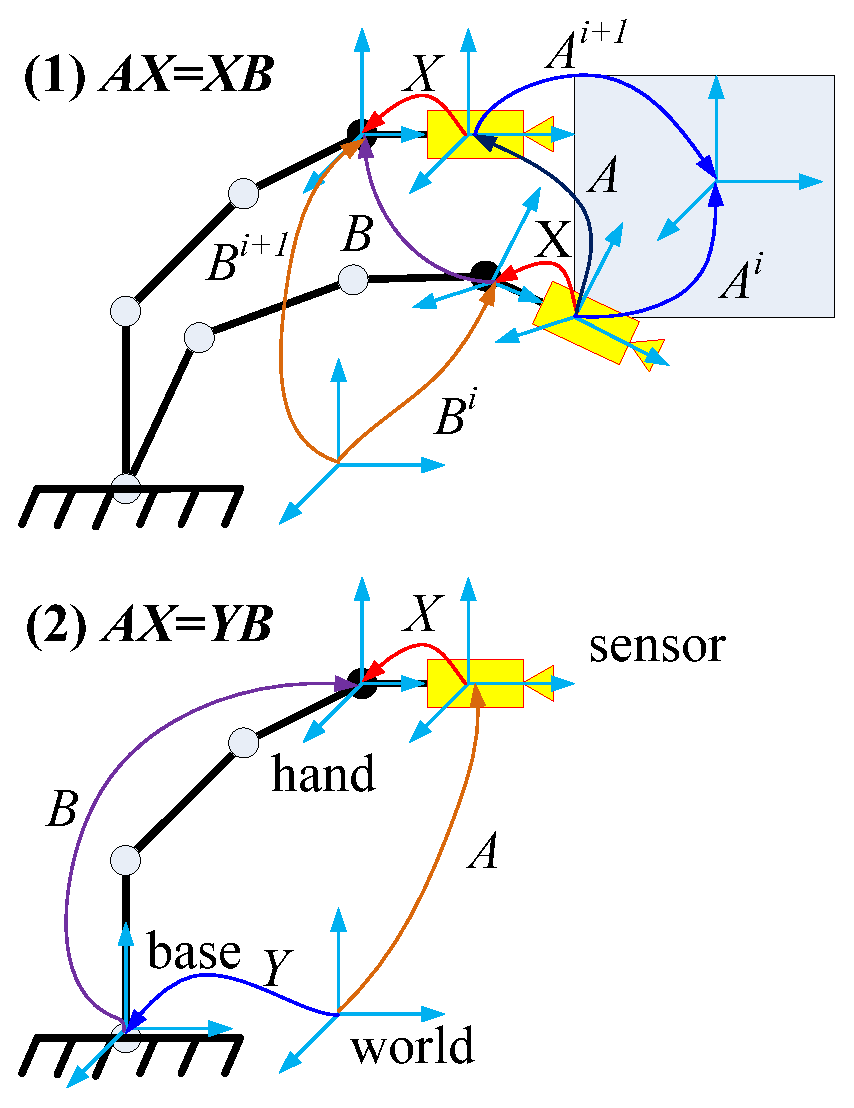
\includegraphics[width=3.2in]{fig1.eps}
\caption{
(1) The hand-eye and robot-robot calibration problem which is formulated as AX=YB. (2) The hand-eye calibration problem which is formulated in a matrix as AX=XB.
}
\label{fig1}
\end{figure}
\end{center}

The hand-eye calibration problem can be generalized as the $\textbf{AX = XB}$ formulation. $A$ and $B$ are respectively the homogeneous transformation matrices of end-effector and sensor movement using $A = A^{i}(A^{i+1})^{-1}; B = B^{i}(B^{i+1})^{-1}$ as shown in Fig.~\ref{fig1}. The homogeneous transformation matrix can be described with the form.
\begin{equation}\label{equ0}
    g(R,t)=\left(
             \begin{array}{cc}
               R & t \\
               0^{T} & 1 \\
             \end{array}
           \right)
\end{equation}

where $R \in SO(3)$ is a rotation matrix and $t \in R^{3}$ is a translation vector.

According to multiple pairs $(A,B) \in SE(3) \times SE(3)$ which are known a prior, many methods for the only $X$ have been proposed including decoupling of rotation and translation, least squares fitting, singular value decomposition (\emph{SVD}), screw theory, nonlinear
optimization, quaternion, gradient descent and interactive approaches \cite{Shiu1989,Tsai1989,Wang1992,Park1994,Horaud1995,Daniilidis1999,Fassi2005,Zhao2011,Ackerman2014a}. Theses methods assume that there is exact knowledge of the $As$ and $Bs$ correspondence. Considering data streams containing the $A$ and $B$ will be asynchronous that are discussed in many instances
in the literature, several methods regardless of the correspondence or recovering the correspondence between two data sets are presented \cite{Ackerman2013a,Ackerman2013,Ackerman2014}.

Simultaneous estimation of the hand-eye transformation and robot-world one
has been viewed as $\textbf{AX=YB}$ problem. As shown in Fig.~\ref{fig1} (1), $Y$ is the transformation of the robot base relative to the world, $A$ is the sensor to the world transformation, and $B$ is the hand/end-effector to the robot base rigid transformation. The $A$ and $B$ in $\textbf{AX=YB}$ calibration is different from ones in $\textbf{AX=XB}$ from a physical view. This problem has been studied in different methods such as SVD, closed-form, quaternion and nonlinear optimization \cite{Zhuang1994,dornaika1998simultaneous,Hirsh2001, ernst2012non,strobl2006optimal,Li2010,Shah2013,Heller2014}. Another approach integrate multiple robots to calibrate hand-eye, tool-flange and robot-robot transformation in $\textbf{AXB=YCZ}$ problem \cite{Wang2014}. Simultaneous solution for $X$ and $Y$ in $\textbf{AX=YB}$ problem is an challenging issue. In the above methods, the correspondence between $A$ and $B$ is known a prior. In this paper, our solution for $\textbf{AX=YB}$ doesn't require a priori knowledge of correspondences.

The rest of the paper is organized as follows. In Section
\ref{sect2} we present the probabilistic theory to solve for $X$ and $Y$. In Section \ref{sect3} a algorithmic solution involving correlation theorem and Euclidean group invariants is posed to recover the correspondence. The simulation results, including unknown correspondence and noisy data stream, are illustrated in Section \ref{sect4}. Finally, we draw some conclusions.

\section{Solving AX=YB using a probabilistic theory on motion groups}
\label{sect2}

Given a large set of pairs $(A_{i},B_{i})\in SE(3)\times SE(3)$ for $i=1,\cdots,n$ that are acquired by measurements and satisfy the following equations

\begin{equation}\label{equ1}
A_{i}X=YB_{i}
\end{equation}

In the case of $SE(3)$, a Dirac delta function, or $\delta$ function, is thought of as a function which is zero everywhere except at the identity where it is infinite.

\begin{equation}\label{equ2}
\delta{(H)}=
\left\{
\begin{array}{ll}
+\infty, & H=I \\
0, & H \neq I
\end{array}
\right.
\end{equation}

Dirac delta function is also constrained to satisfy the identity.

\begin{equation}\label{equ3}
\int_{SE(3)}\delta{(H)}dH=1
\end{equation}

A shifted Dirac delta function can be defined as $\delta_{A}(H)=\delta{(A^{-1}H)}$. Given two functions $f_{1}(g)$ and $f_{2}(g)$, their convolution in Lie group is defined as follows,

\begin{equation}\label{equ4}
(f_{1}\ast f_{2})(g)=\int_{SE(3)}f_{1}(h)f_{2}(h^{-1}\circ g)dh
\end{equation}

Considering the properties of $\delta$ function, the following equation is built.

\begin{equation}\label{equ5}
(f\ast \delta)(g)=\int_{SE(3)}f(h)\delta(h^{-1}\circ g)dh=f(g)
\end{equation}

Therefore, for each $A_{i}$ and $B_{i}$, we can get

\begin{IEEEeqnarray}{l}\label{equ6}
(\delta_{A_{i}}\ast \delta_{X})(g)=\delta(A_{i}^{-1} g X^{-1}) \IEEEyessubnumber
\\*
(\delta_{Y}\ast \delta_{B_{i}})(g)=\delta(Y^{-1} g B_{i}^{-1}) \IEEEyessubnumber
\end{IEEEeqnarray}

Together with $g=A_{i}X=YB_{i}$, we can obtain the convolution equation

\begin{equation}\label{equ7}
(\delta_{A_{i}}\ast \delta_{X})(g)=(\delta_{Y}\ast \delta_{B_{i}})(g)
\end{equation}

Convolution provides a linear operation on functions with additional properties. We can add up $n$ instances into a single function.

\begin{IEEEeqnarray}{l}\label{equ8}
f_{A}(g)=\frac{1}{n}\sum_{i=1}^{n} \delta(A_{i}^{-1}g) \IEEEyessubnumber
\\*
f_{B}(g)=\frac{1}{n}\sum_{i=1}^{n} \delta(B_{i}^{-1}g) \IEEEyessubnumber
\end{IEEEeqnarray}

Therefore,

\begin{equation}\label{equ9}
(f_{A_{i}}\ast \delta_{X})(g)=(\delta_{Y}\ast f_{B_{i}})(g)
\end{equation}

In each transformation set $A_i$s and $B_i$s, we are using small relative motions between consecutive reference frames. Given a measure of distance between reference frames, e.g.

\begin{eqnarray}\label{equ10}
d^{2}(A_{i},A_{j})=\parallel \Delta A \parallel_{W}^{2} = trace[(\Delta A)W(\Delta A)^{T}] = \epsilon,\nonumber \\
\end{eqnarray}

we have that  $\Delta A = A_{i}-A_{j}$ and $0 < \epsilon \ll 1 $

The convolution of "highly focused" distributions corresponding to closely clumped sets of reference frames have some interesting properties that we can exploit to solve for $X$. In particular, let the mean and covariance of a probability density, $f(g)$(e.g. $f_{A}(g),f_{B}(g)$), be defined by the conditions.


\begin{IEEEeqnarray}{l}\label{equ11}
\int_{SE(3)}log(M^{-1}g))f(g)dg=0 \IEEEyessubnumber
\\*
\Sigma = \int_{SE(3)}log^{\vee}(M^{-1}g)[log^{\vee}(M^{-1)}g)]^{T}f(g)dg \IEEEyessubnumber
\end{IEEEeqnarray}

A discrete version as for $f_{A}(g)$ is

\begin{IEEEeqnarray}{l}\label{equ12}
\sum_{i=1}^{n}log(M^{-1}g))=0 \IEEEyessubnumber
\\*
\Sigma_{A} = \sum_{i=1}^{n}log^{\vee}(M^{-1}g)[log^{\vee}(M^{-1)}g)]^{T} \IEEEyessubnumber
\end{IEEEeqnarray}

While the cloud of frames ${A_{i}}$ is clustered around $M_{A}$, an iterative formula can be used for computing $M_{A}$ \cite{Wang2008}.

\begin{equation}\label{equ13}
    ^{k+1}M_{A} = ^{k}M_{A} \circ exp[\frac{1}{n}\sum_{i=1}^{n}log(^{k}M_{A}^{-1}\circ A_{i})]
\end{equation}

An initial estimate of the iterative procedure can be $^{0}M_{A}=\frac{1}{n}\sum_{i=1}^{n}log(A_{i})$, then the process iterates until the cost function, $\parallel \sum_{i=1}^{n}log(M_{A}^{-1}A_{i}) \parallel^{2}$ falls below a predefined threshold, where the cost function is minimized and the minimum defines $M_{A}$. A similar procedure is used for computing $M_B$.

The mean and covariance for the convolution $(f_{1} \ast f_{2})(g)$ of two highly focused functions, $f_{1}$ and $f_{2}$ can be computed as

\begin{IEEEeqnarray}{l}\label{equ14}
M_{1 \ast 2} = M_{1}M_{2} \IEEEyessubnumber
\\*
\Sigma_{1 \ast 2} = Ad(M_{2}^{-1})\Sigma_{1}Ad^{T}(M_{2}^{-1}) + \Sigma_{2} \IEEEyessubnumber
\end{IEEEeqnarray}

where

$$Ad(g)=\left(
               \begin{array}{cc}
                 R & O \\
                 \hat{t}R & R \\
               \end{array}
             \right)$$

Because $X$ and $Y$ is fixed, as for $\delta_{X}(g)$ and $\delta_{Y}(g)$, mean and covariance are $M_{X}=X$, $\Sigma_{X}=0$ and $M_{Y}=Y$, $\Sigma_{Y}=0$, respectively, therefore we can obtain

\begin{IEEEeqnarray}{l}
M_{A} X = Y M_{B} \IEEEyessubnumber\label{equ15a}
\\*
Ad(X^{-1})\Sigma_{A}Ad^{T}(X^{-1}) = \Sigma_{B} \IEEEyessubnumber\label{equ15b}
\end{IEEEeqnarray}

From (\ref{equ15a}), we can obtain

\begin{IEEEeqnarray}{l}
R_{M_{A}} R_{X} = R_{Y} R_{M_{B}} \IEEEyessubnumber\label{equ16a}
\\*
R_{M_{A}} t_{X} + t_{M_{A}}= R_{Y} t_{M_{B}} + t_{Y} \IEEEyessubnumber\label{equ16b}
\end{IEEEeqnarray}

$\Sigma_{M_{A}}$ and $\Sigma_{M_{B}}$ can be decomposed into blocks as
$\left(\begin{array}{cc}
       \Sigma_{M_{A}}^{1} & \Sigma_{M_{A}}^{2} \\
       \Sigma_{M_{A}}^{3} & \Sigma_{M_{A}}^{4} \\
       \end{array}
       \right)$
and
$\left(\begin{array}{cc}
       \Sigma_{M_{B}}^{1} & \Sigma_{M_{B}}^{2} \\
       \Sigma_{M_{B}}^{3} & \Sigma_{M_{B}}^{4} \\
       \end{array}
       \right)$, respectively. Using
$ X^{-1}=X^{T}=\left(\begin{array}{cc}
       R_{X}^{T} & -R_{X}^{T}t_{X}  \\
       0 & 1 \\
       \end{array}
       \right)$,
then we can write the first two blocks of (\ref{equ15b}) as follows,

\begin{IEEEeqnarray}{l}
\Sigma_{M_{B}}^{1} = R_{X}^{T}\Sigma_{M_{A}}^{1} R_{X} \IEEEyessubnumber\label{equ17a}
\\*
\Sigma_{M_{B}}^{2} = R_{X}^{T}\Sigma_{M_{A}}^{1} R_{X} (\widehat{R_{X}^{T}t_{X}}) + R_{X}^{T}\Sigma_{M_{A}}^{2}R_{X}
 \IEEEyessubnumber\label{equ17b}
\end{IEEEeqnarray}

The first blocks (\ref{equ17a}) is eigendecomposed with the same diagonal matrix due to matrix similarity $\Sigma_{M_{A}}^{1}=Q_{M_{A}}\wedge Q_{M_{A}}^{T}$, $\Sigma_{M_{B}}^{1}=Q_{M_{B}}\wedge Q_{M_{B}}^{T}$. Then,

\begin{equation}\label{equ18}
    \wedge = (Q_{M_{A}}^{T}R_{X}Q_{M_{B}}) \wedge (Q_{M_{B}}^{T}R_{X}^{T}Q_{M_{A}})= P \wedge P^{T}
\end{equation}

In $P=Q_{M_{A}}^{T}R_{X}Q_{M_{B}}$, $Q_{M_{A}}$ and $Q_{M_{B}}$ are constrained to be a rotation matrix and therefore $P \in \Omega \bigcup (-\Omega)$,

\begin{equation}\label{equ19}
\Omega= \left(
\begin{array}{ccc}
\left( \begin{array}{ccc}
       1 & 0 & 0 \\
       0 & 1 & 0 \\
       0 & 0 & 1 \\
\end{array} \right),&
\left( \begin{array}{ccc}
       -1 & 0 & 0 \\
       0 & -1 & 0 \\
       0 & 0 & 1 \\
\end{array} \right)
\\
\left( \begin{array}{ccc}
       -1 & 0 & 0 \\
       0 & 1 & 0 \\
       0 & 0 & -1 \\
\end{array} \right),&
\left( \begin{array}{ccc}
       1 & 0 & 0 \\
       0 & -1 & 0 \\
       0 & 0 & -1 \\
\end{array} \right)
\end{array}
\right)
\end{equation}

Therefore, there are eight possibilities of $R_{X}, R_{X}=Q_{M_{A}}PQ_{M_{B}}^T$. Then, from \ref{equ17b}, eight $t_{X}$ corresponding to $R_{X}$ can be directly found. Furthermore, eight candidate $R_{Y} and t_{Y}$ can be found. At last, there are eight possibilities of solution $(X_{i},Y_{i}), i = 1,\dots,8$.
where,

\begin{equation}\label{equ20}
\begin{array}{cc}
X_{i}= \left( \begin{array}{cc}
       R_{X} & t_{X} \\
       \mathbf{0}^{T} & \mathbf{1}\\
\end{array} \right),&
Y_{i}= \left( \begin{array}{cc}
       R_{Y} & t_{Y} \\
       \mathbf{0}^{T} & \mathbf{1}\\
\end{array} \right)
\end{array}
\end{equation}

Based on the screw theory, it is known that a homogeneous transformation $H$ can be written in the form with four parameters $(\theta,d,\mathbf{n},\mathbf{p})$.

\begin{equation}\label{equ21}
H = \left( \begin{array}{cc}
       e^{\theta \hat{\mathbf{n}}} & (\mathbf{I}_{3} - e^{\theta \hat{\mathbf{n}}})\mathbf{p} + d\mathbf{n} \\
       \mathbf{0}^{T} & \mathbf{1}
\end{array} \right)
\end{equation}

$AX=YB$ can be written as $AX=X(X^{-1}YB)$ and let $B' = X^{-1}YB$ . In the form $AX=XB'$, there exit two Euclidean-Group invariant relationships for one of eight groups of $(A_{i},B_{i}^k)( i = 1,\cdots,n; k=1,\dots,8), B_i^{k} = X^{-1}YB_i$ as follows,

\begin{equation}\label{equ22}
    \theta_{A_{i}}=\theta_{B_{i}^{k}}, d_{A_{i}}=d_{B_{i}^{k}}
\end{equation}

From among the four pairs $(X_{i},Y_{i})$, we can find a correct solution to minimize the absolute deviations,

\begin{equation}\label{equ23}
    (X,Y) = \mathop{\mathbf{arg}min}_{(X_{i},Y_{i})}\frac{1}{n} \sum_{i=1}^{n} (\parallel \theta_{A_{i}}-\theta_{B_{i}^{k}} \parallel + \parallel d_{A_{i}}-d_{B_{i}^{k}} \parallel)
\end{equation}

\section{Solution with unknown correspondence of $A_{i}$ and $B_{i}^{k}$}
\label{sect3}

In most cases, the homogeneous transformations with $As$ and $Bs$ are given based on the data from different sensors. Due to asynchronous timing of the measurement transmissions, the correspondences between $A_{i}$ and $B_{i}^{k}$ is unknown. The advantage of the above probabilistic solution lies on that $X$ and $Y$ can be calculated even if without any a priori knowledge of the correspondence. However, there are still eight possible candidate results $(X_{i},Y_{i})$. Using Euclidean-Group invariants, it is straightforward to determine which pair is the correct one if the correspondence between $A_{i}$ and $B_{i}^{k}$ can be known.

The Discrete Fourier Transform (DFT) decomposes a time-domain signal into its constituent frequencies. The input is a finite list of equally spaced samples of a function. Given a discrete signal consisting of a sequence of $N$ complex numbers $x_{0},x_{1},\cdots,x_{N-1}$, the DFT is denoted by $X_{\kappa} = \mathcal{F}{x_{n}}$

\begin{equation}\label{equ21}
    X_{\kappa} = \sum_{n=0}^{N-1}x_{n}\cdot exp(-i\frac{2\pi}{N}n\kappa)
\end{equation}
The Inverse Discrete Fourier transform (IDFT) denoted by

\begin{equation}\label{equ22}
    x_{n} = \frac{1}{N}\sum_{n=0}^{N-1}X_{\kappa}\cdot exp(i\frac{2\pi}{N}n\kappa)
\end{equation}

The discrete convolution of two sequences $f_{n}$ and $g_{n}$  are defined

\begin{equation}\label{equ23}
    (f \ast g)(\tau)=\sum_{i=0}^{N}f(t_{i})g(t_{i}-\tau)
\end{equation}

In convolution theorem, the Fourier transform of a convolution is the product of the Fourier transforms, namely,

\begin{equation}\label{equ24}
    f \ast g = \mathcal{F}^{-1} [\mathcal{F}(f) \cdot \mathcal{F}(g)]
\end{equation}

The correlation theorem indicates that the correlation function, $Corr(f,g)$, will have a large value at a shift vector if the two sequences $f$ and $g$ contain similar features. The correlation can be obtained based on the convolution theorem. The DFT of the correlation $Corr(f,g)$ is equal to the product of the DFT of a sequence $f_{n}$ and the complex conjugate $\mathcal{F}^{*}$ of the DFT of the other sequence $g_n$.

\begin{equation}\label{equ25}
    Corr(f,g)=f \star g = \mathcal{F}^{-1}[\mathcal{F}(f) \cdot (\mathcal{F}(g))^{*}]
\end{equation}

Compared with the standard time-domain convolution algorithm, the complexity of the convolution by multiplication in the frequency domain is significantly reduced with the help of the convolution theorem and the fast Fourier transform (FFT).

There are two sequences $\theta_{A_{i}}$ and $\theta_{B_{i}^{k}}$ from each pair $(A_{i},B_{i}^{k})$. For homogeneous transformations from which the range of $\theta$ can vary, two sequences $\theta_{Ai}$ and $\theta_{B_{i}^{k}}$ can be first normalized.

\begin{equation}\label{equ26}
    \theta_{1}=\frac{(\theta_{A_{i}}-\mu_{A_{i}})}{\sigma_{A_{i}}}, \theta_{2}=\frac{(\theta_{B_{i}^{k}}-\mu_{B_{i}^{k}})}{\sigma_{B_{i}^{k}}}
\end{equation}

where $\mu_{A_{i}}(\mu_{B_{i}^{k}})$ is the average of $\theta_{A_{i}}(\theta_{B_{i}^{k}})$ and $\sigma_{A_{i}}(\sigma_{B_{i}^{k}})$ is the standard deviation.

Here, the correlation function $Corr(\theta_{1},\theta_{2})$  is the function of the time sequence index $(n)$ which describes the probability that these two sequences are separated by this particular unit. The location of the function maximum indicates the amount of shift, $\tau_{shift}$, between the two sequence $\theta_{A_{i}}$ and $\theta_{B_{i}^{k}}$.

\begin{equation}\label{equ27}
    \tau_{shift} = \mathop{\mathbf{arg}max}_{index}(Corr(\theta_{1},\theta_{2}))
\end{equation}

Therefore, the correspondence between the two sequences can be found. The data of $\theta_{A_{i}}$ or $d_{A_{i}}$ are shifted by $-\tau_{shift}$ to obtain a sequence of new pairs $(\theta_{A_{i}}(i+\tau_{shift}),\theta_{B_{i}^{k}})$ and $(d_{A_{i}}(i+\tau_{shift}),d_{B_{i}^{k}})$, $max(i,i+\tau_{shift})\leq i \leq min(i,i+\tau_{shift})$. The data stream can be shifted to reach correspondence once the shift is found and the correct solution can also be found by minimizing the absolute deviations based on Euclidean-Group invariants relations using the method in Section \ref{sect2}.


\section{Simulation Studies}
\label{sect4}

\begin{center}
\begin{figure}
\centering
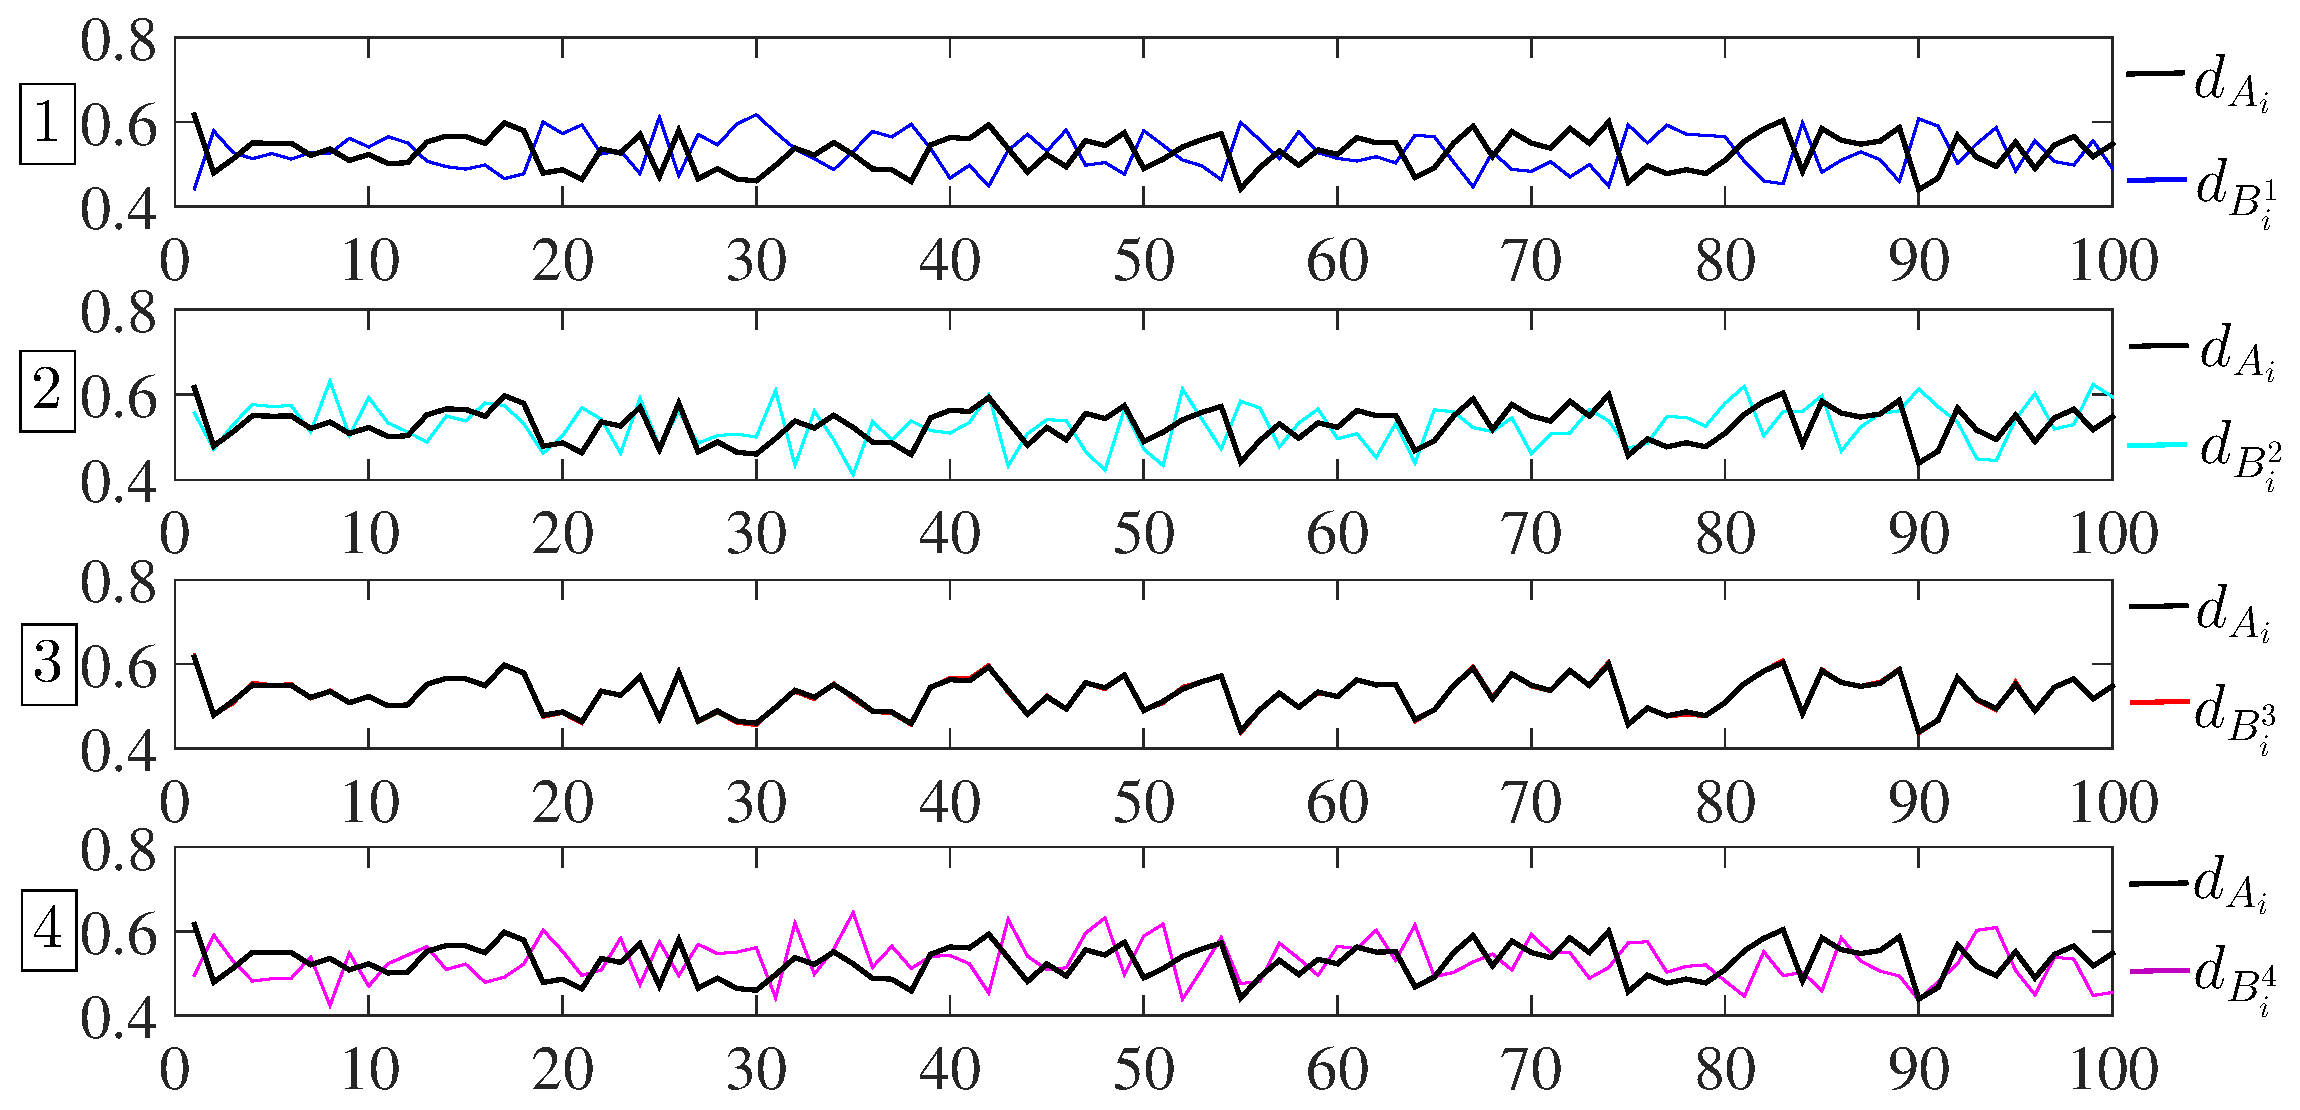
\includegraphics[width=2.6in]{fig3.eps}
\caption{
$Bs$ are randomly generated using  $B_i=B_{init}exp(\widehat{\mathbf{x}})$,$\mathbf{x}=(x_1,\dots,x_6)^T $ \ $x_i \sim \mathcal{N}(0,0.1)$.
}
\label{fig2}
\end{figure}
\end{center}

\begin{figure}
\centering
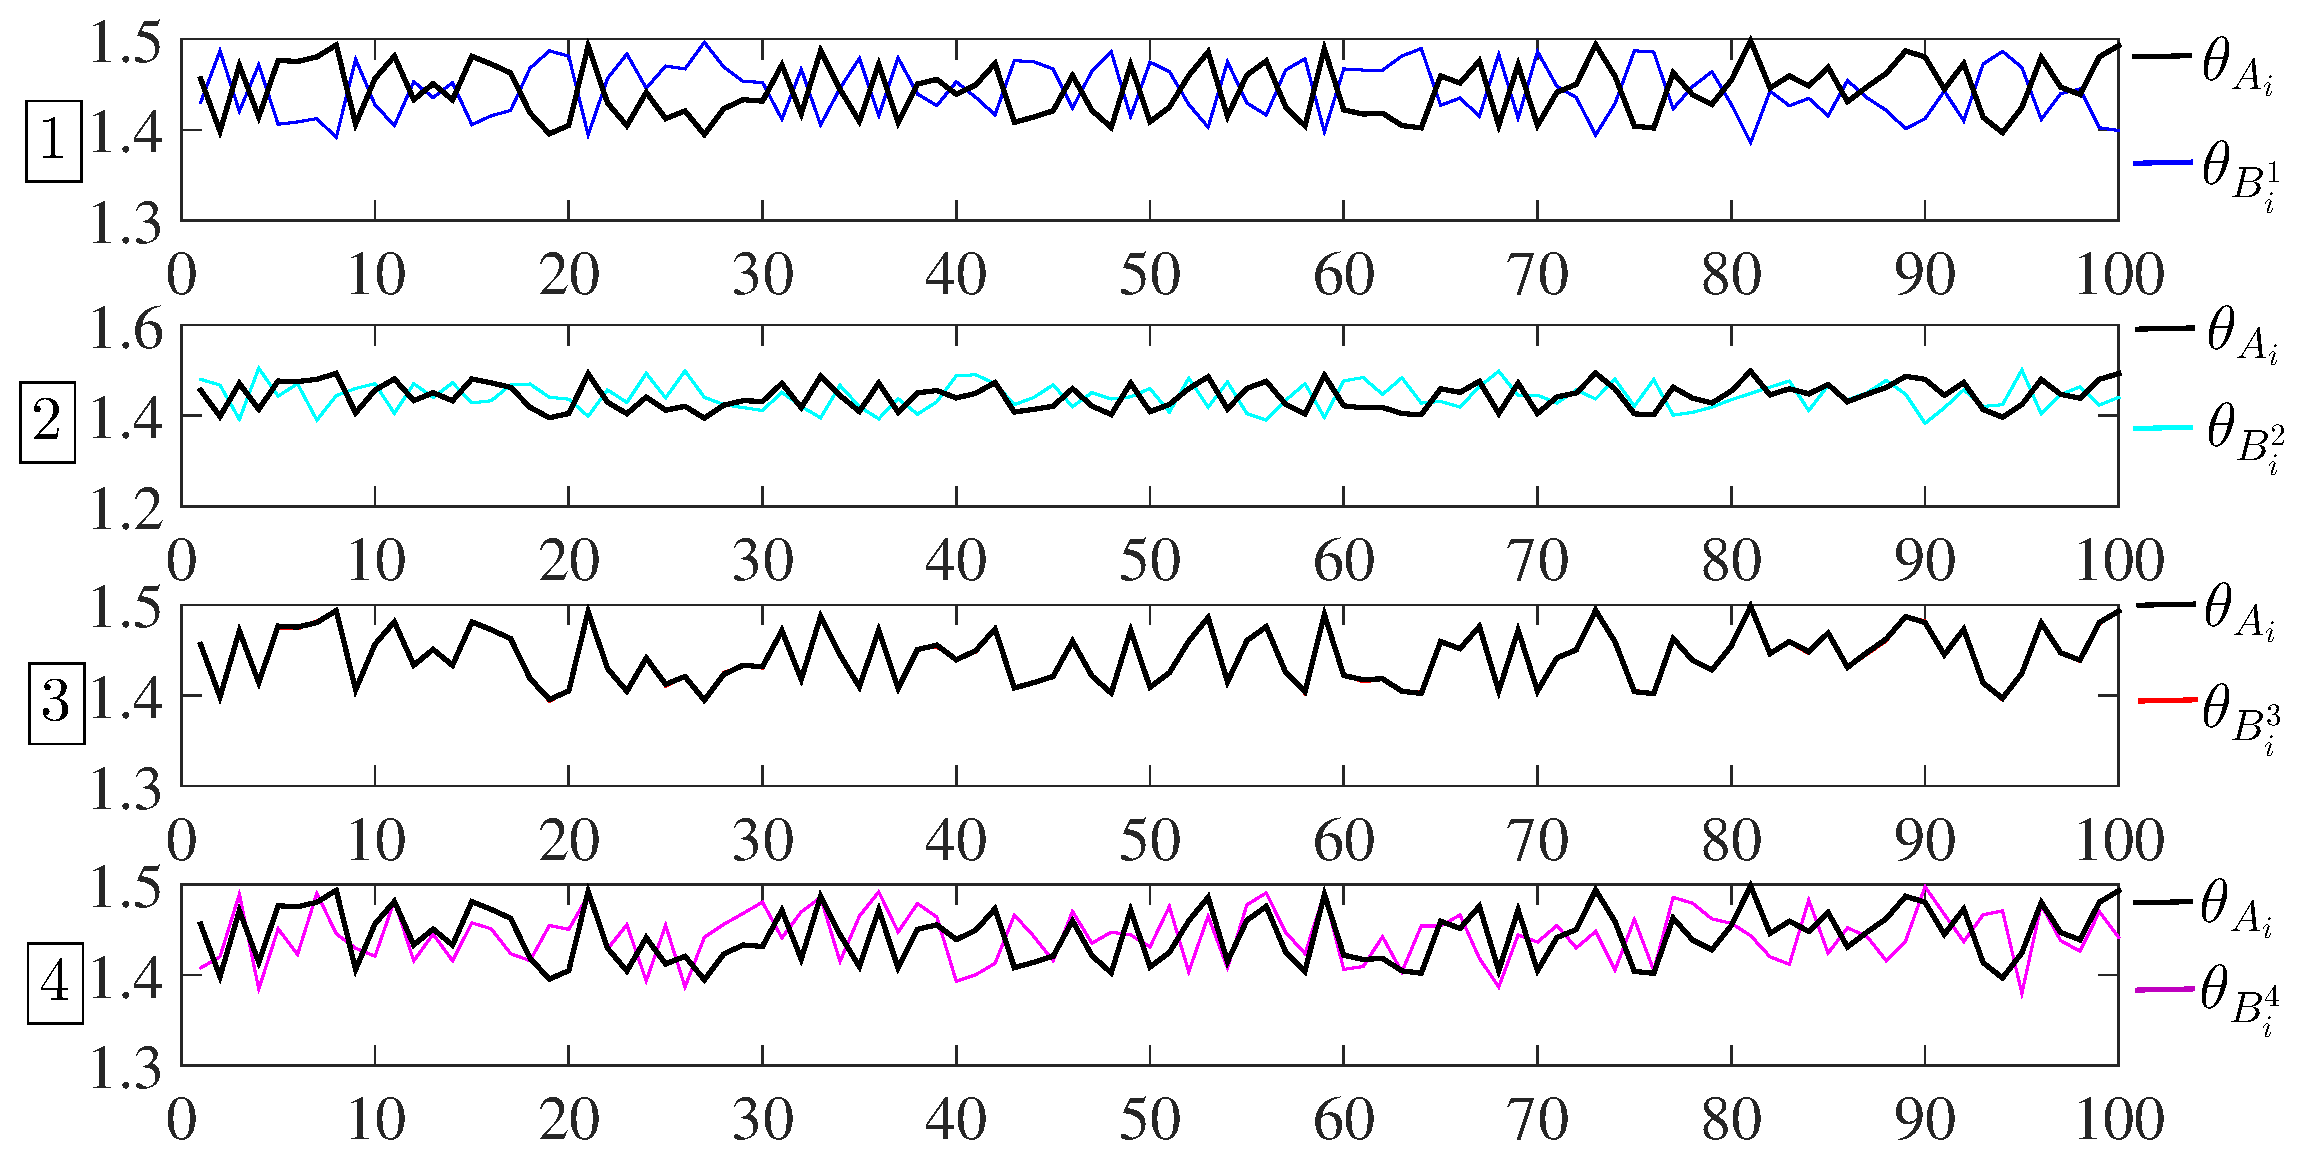
\includegraphics[width=2.6in,bb=84 202 501 581]{fig2.eps}
\caption{
$As$ are calculated using $AX=YB$. $X$ and $Y$ are assumed.
}
\label{fig3}
\end{figure}


In the numerical experiments in this section, the rotational and translational error for $X$ and $Y$ are measured as  $Error(R_X) = \parallel log^{\vee} (R_{X_{Solved}}^{T}R_{X_{true}})\parallel$, $Error(t_X) = \parallel (t_{X_{Solved}}-t_{X_{true}})\parallel$, $Error(R_Y) = \parallel log^{\vee} (R_{Y_{Solved}}^{T}R_{Y_{true}})\parallel$ and $Error(t_Y) = \parallel (t_{Y_{Solved}}-t_{Y_{true}})\parallel$ respectively.

\begin{center}
\begin{figure}
\centering
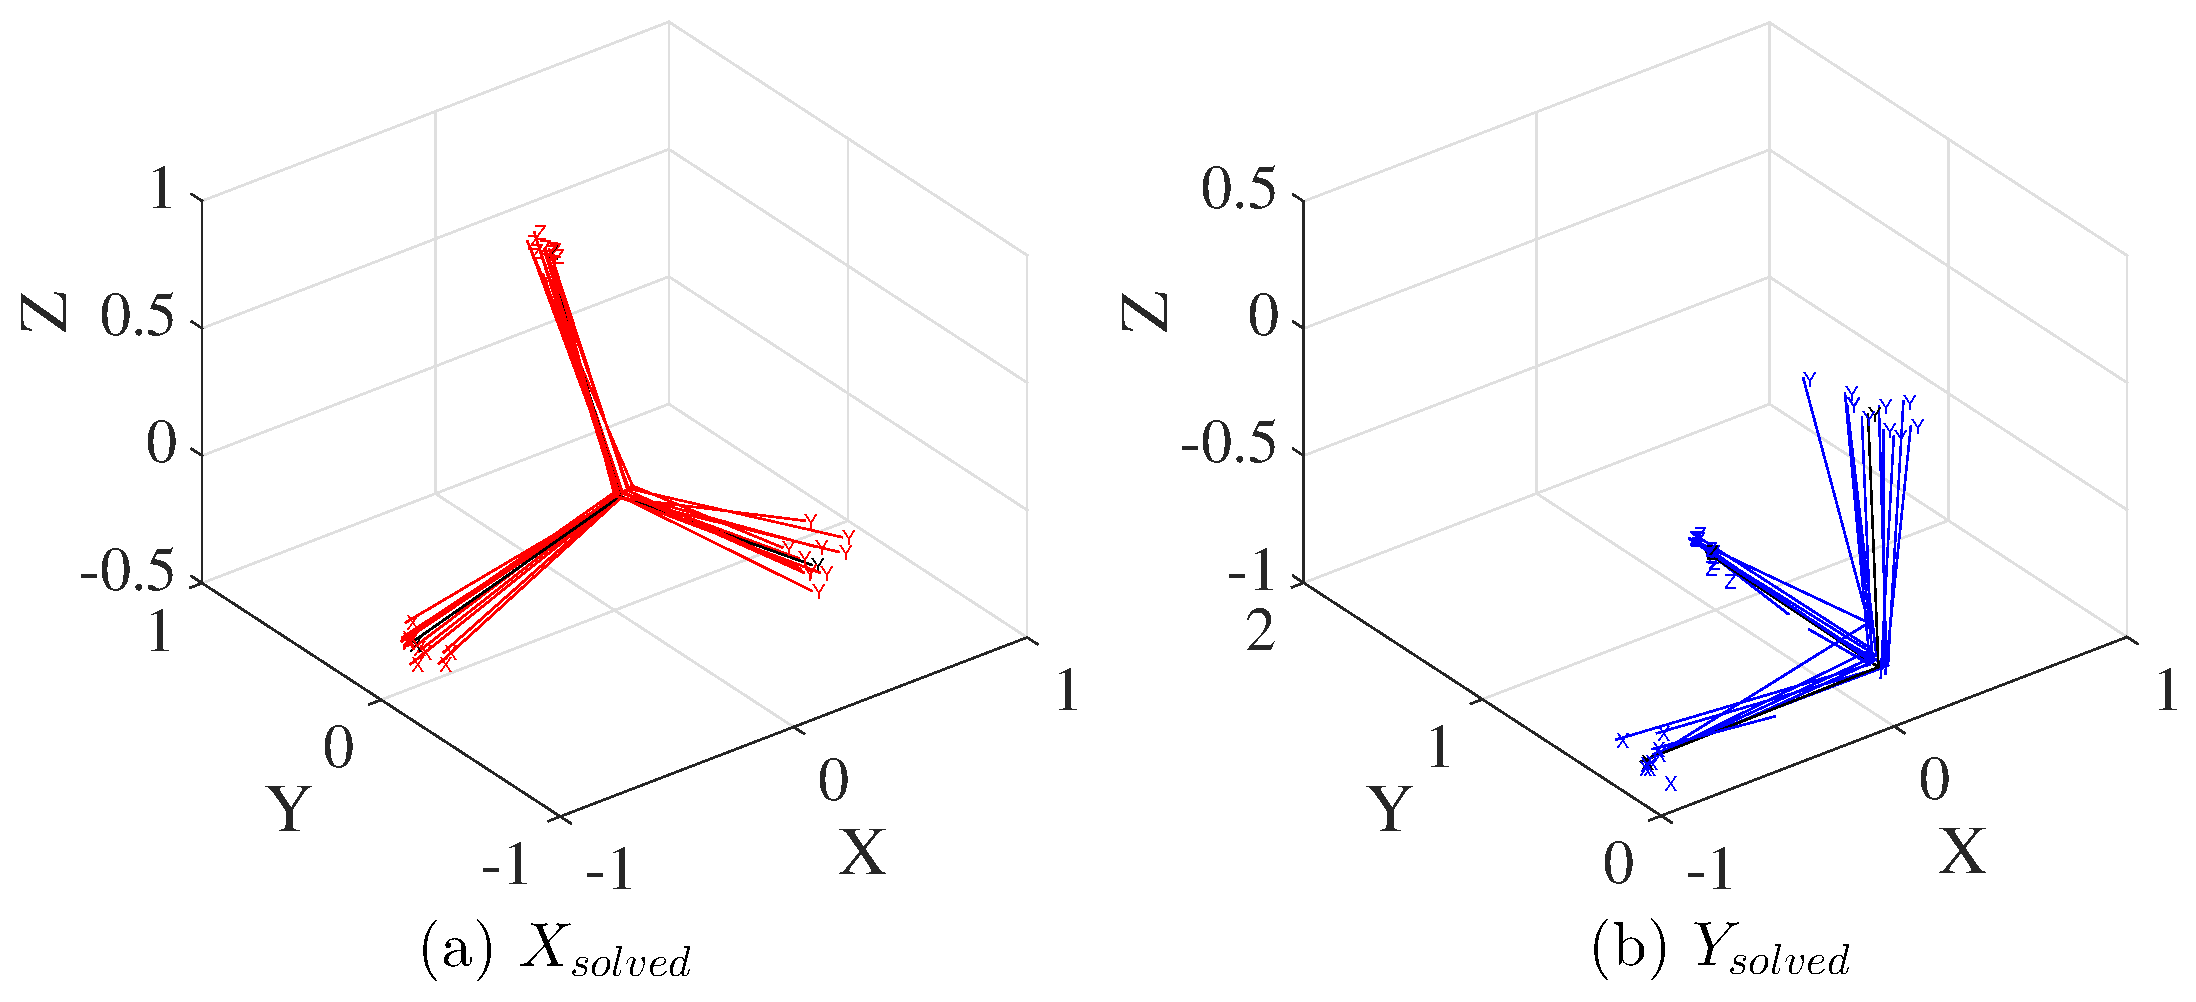
\includegraphics[width=3.2in]{fig4.eps}
\caption{
The cross correlation of data streams of $(A_{i},B_{i}^{k})$ respectively.
}
\label{fig4}
\end{figure}
\end{center}

\begin{center}
\begin{figure}
\centering
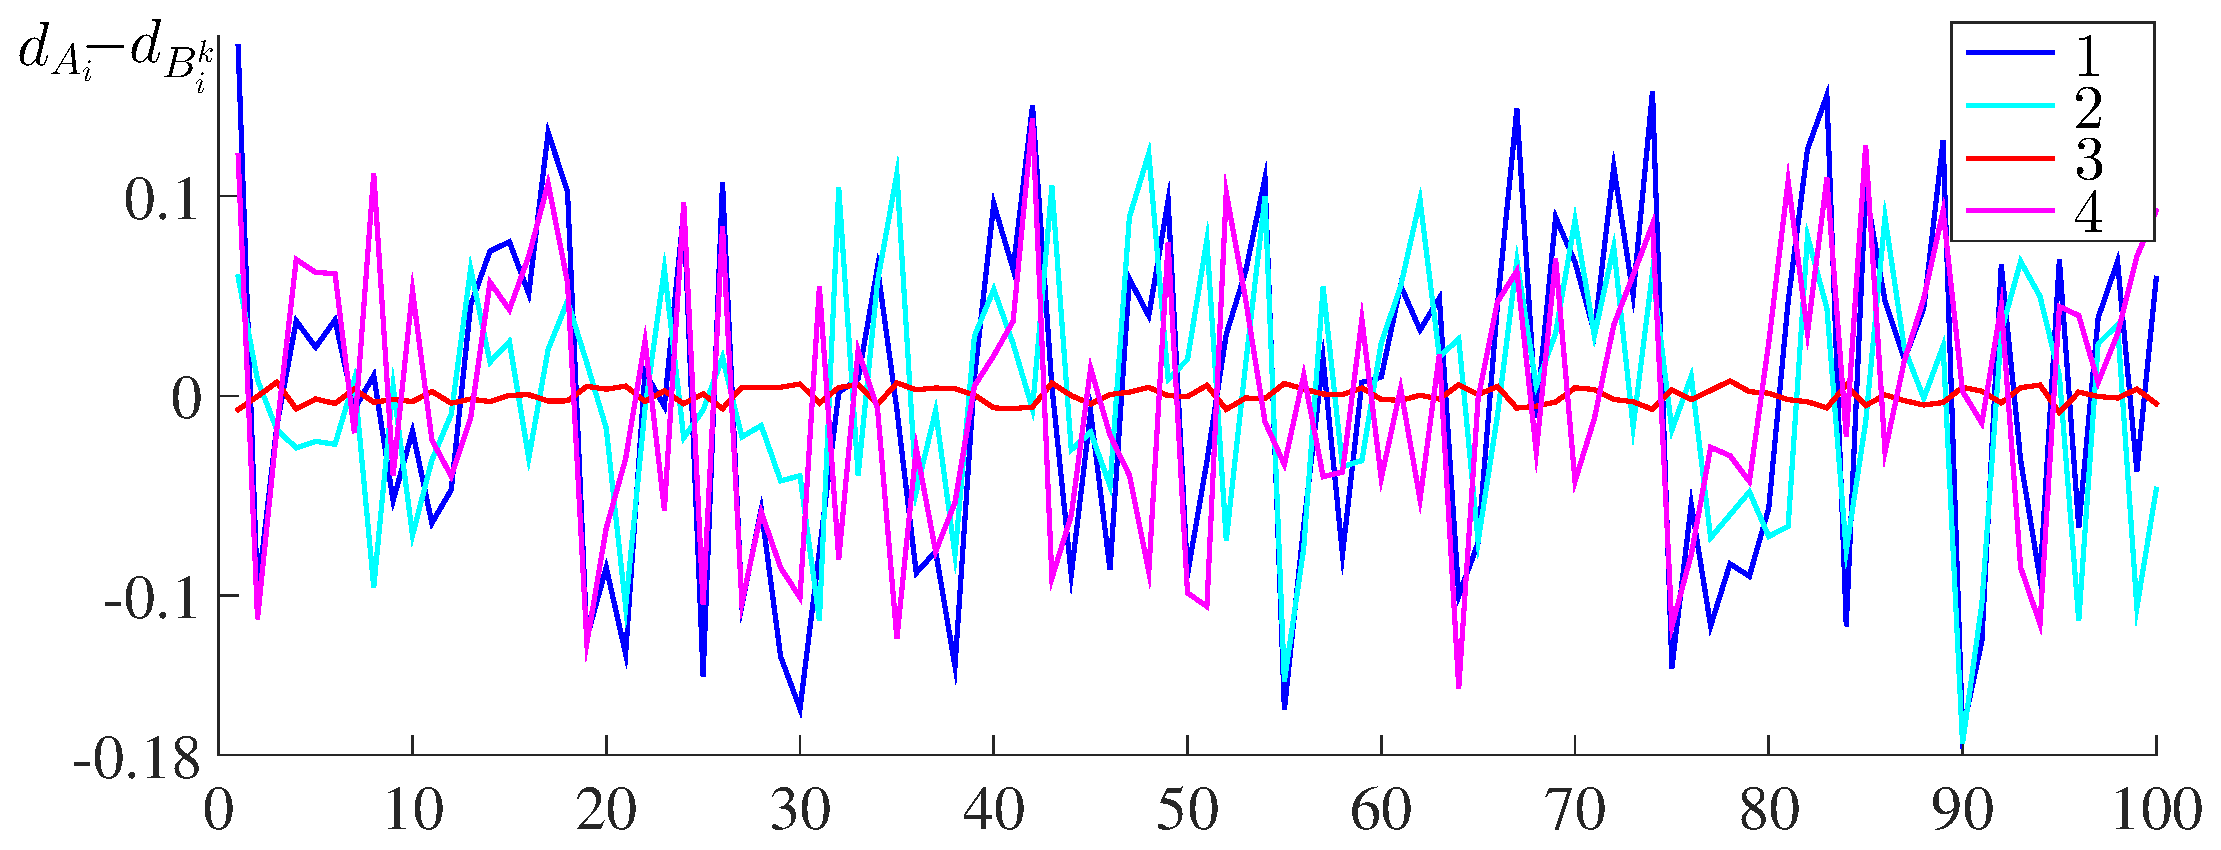
\includegraphics[width=3.2in]{fig5.eps}
\caption{
Calculated rotational and translational deviation of $X$ and $Y$ solved using the data in Fig.~\ref{fig2} and Fig.~\ref{fig3}.
}
\label{fig5}
\end{figure}
\end{center}


$B_{i}$ are generated randomly closely around $B_{init}$ using $B_i = B_{init} exp(\mathbf{\widehat{x}})$ and $i$ pose measurements were employed for generating $i$ $A_{i}$ by $A_{i} = YB_{i}X^{-1}$ as shown in Fig.~\ref{fig2} in which a example shows $A$ and $B$ distribution. As a result by applying the above probabilistic method, 8 sequences $(\theta_{A_{i}},\theta_{B_{i}^{k}})$ and $(d_{A_{i}},d_{B_{i}^{k}})$ $ (i=5,\cdots, 100, k=1,\dots,8)$ can be obtained respectively.

If the data streams of $As$ were shifted by $m$ units compared to the data stream $Bs$. The maximum of cross correlation can be used to find the corresponding shift, which is $-m$ shown in Fig.~\ref{fig4}, representing the data stream of $B_{i}^{k}$ has been shifted by -m units with respect to ${A_{i}}$. Therefore, we shift the data stream inversely to recover the correspondence for finding a correct solution satisfying Euclidean-Group invariants.


Using the minimum sum of $||\theta_{A_{i}} - \theta_{B_{i}^{k}}||$ and $||d_{A_{i}} - d_{B_{i}^{k}}||$, we can find the ${B_{i}^{k}}(k=3)$ corresponding to the least sum of errors and then, only a $(X_k,Y_k)$ is the desired solution. In Fig.~\ref{fig5}, as the number of $(A,B)$ pairs increase, the errors of translation and rotations are reduced but when the number comes to a certain value, the errors cannot be reduced furthermore.

\begin{center}
\begin{figure}
\centering
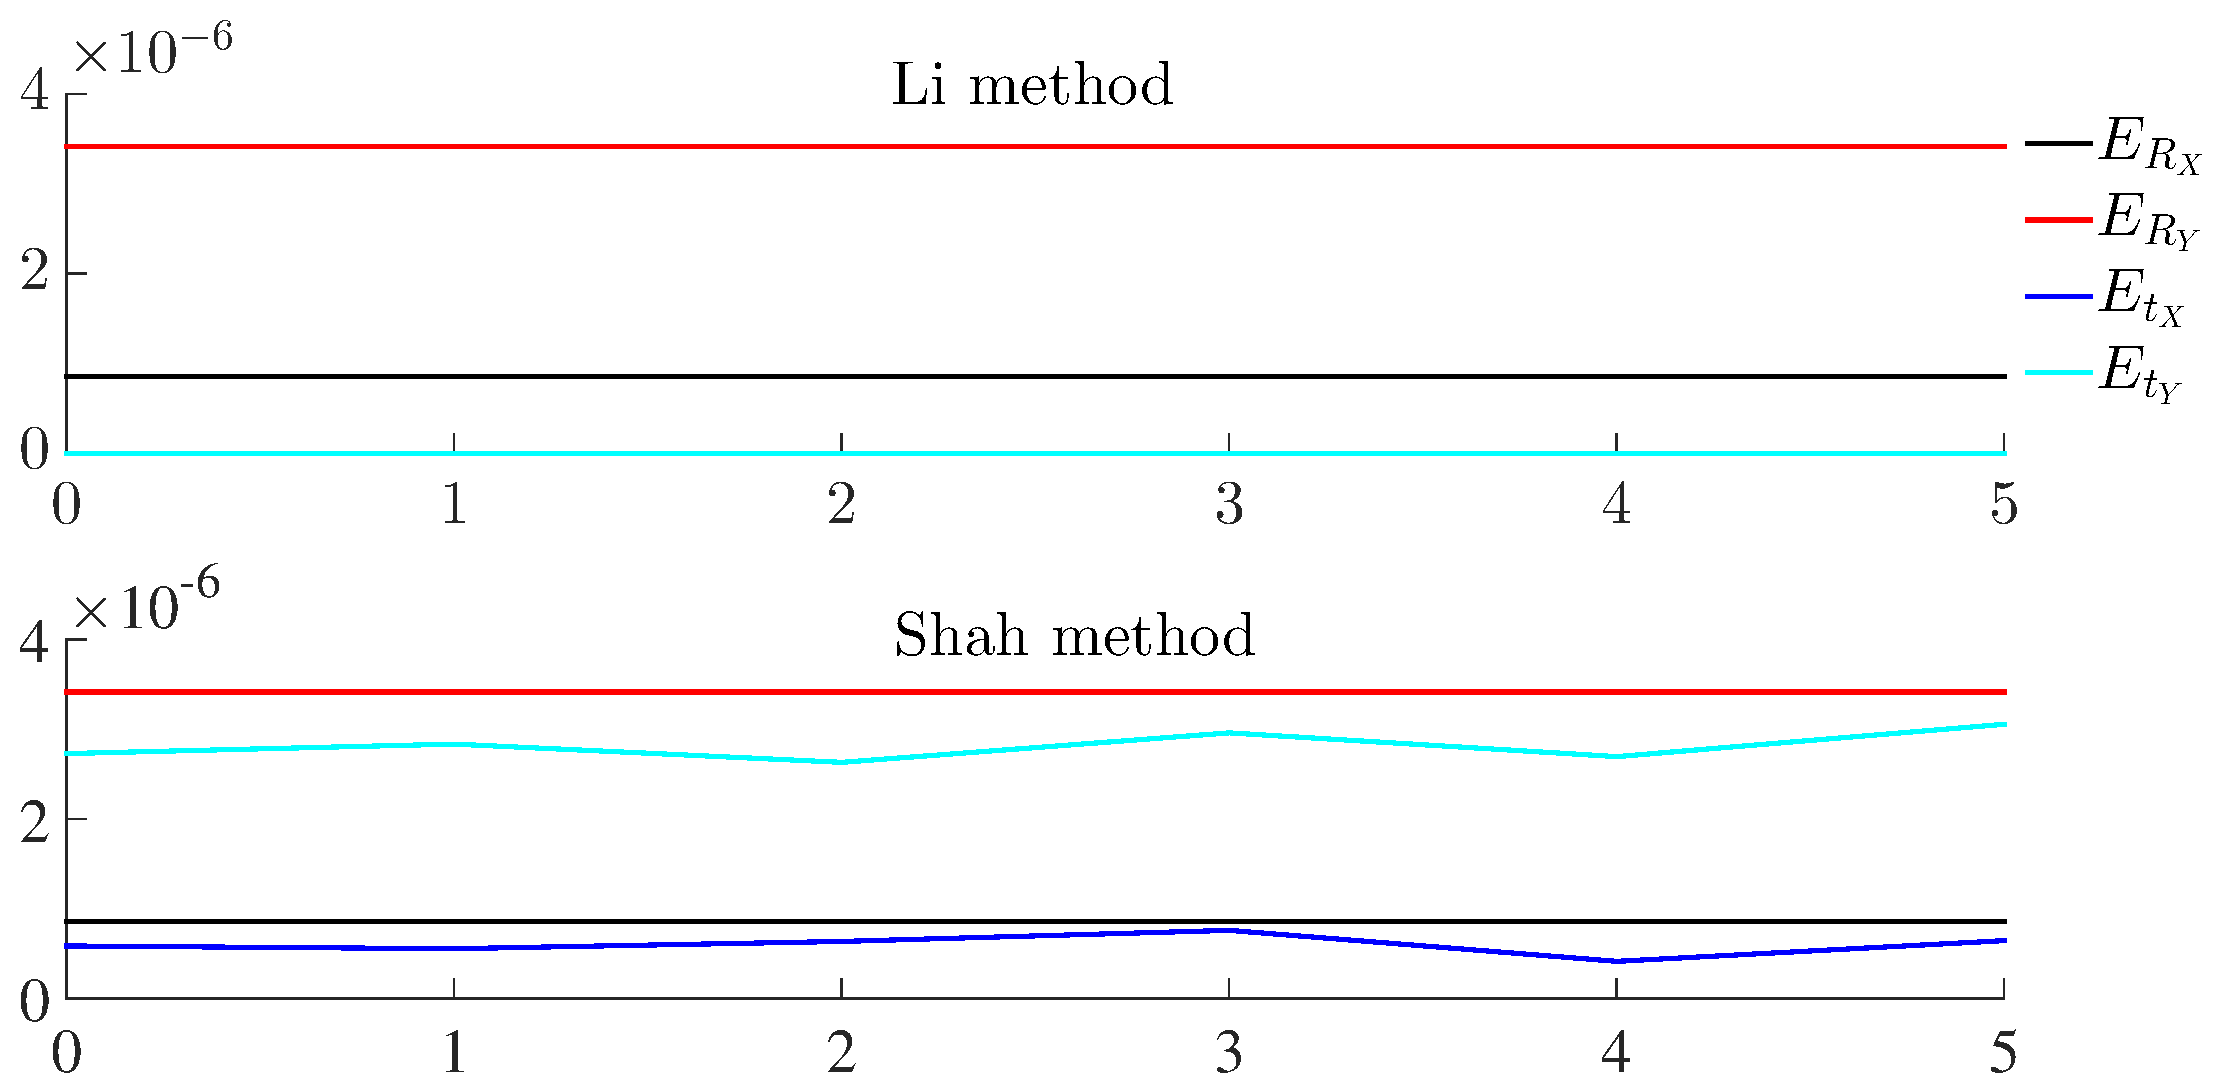
\includegraphics[width=3.2in]{fig6.eps}
\caption{
$Error(R_X)$ distribution as the $As$ and $Bs$ spread ($\sigma(x_i) = 0.1, 0.2, 0.4, 0.6, 0.8, 1, 2$ as shown in Fig.~\ref{fig2})
}
\label{fig6}
\end{figure}
\end{center}

\begin{center}
\begin{figure}
\centering
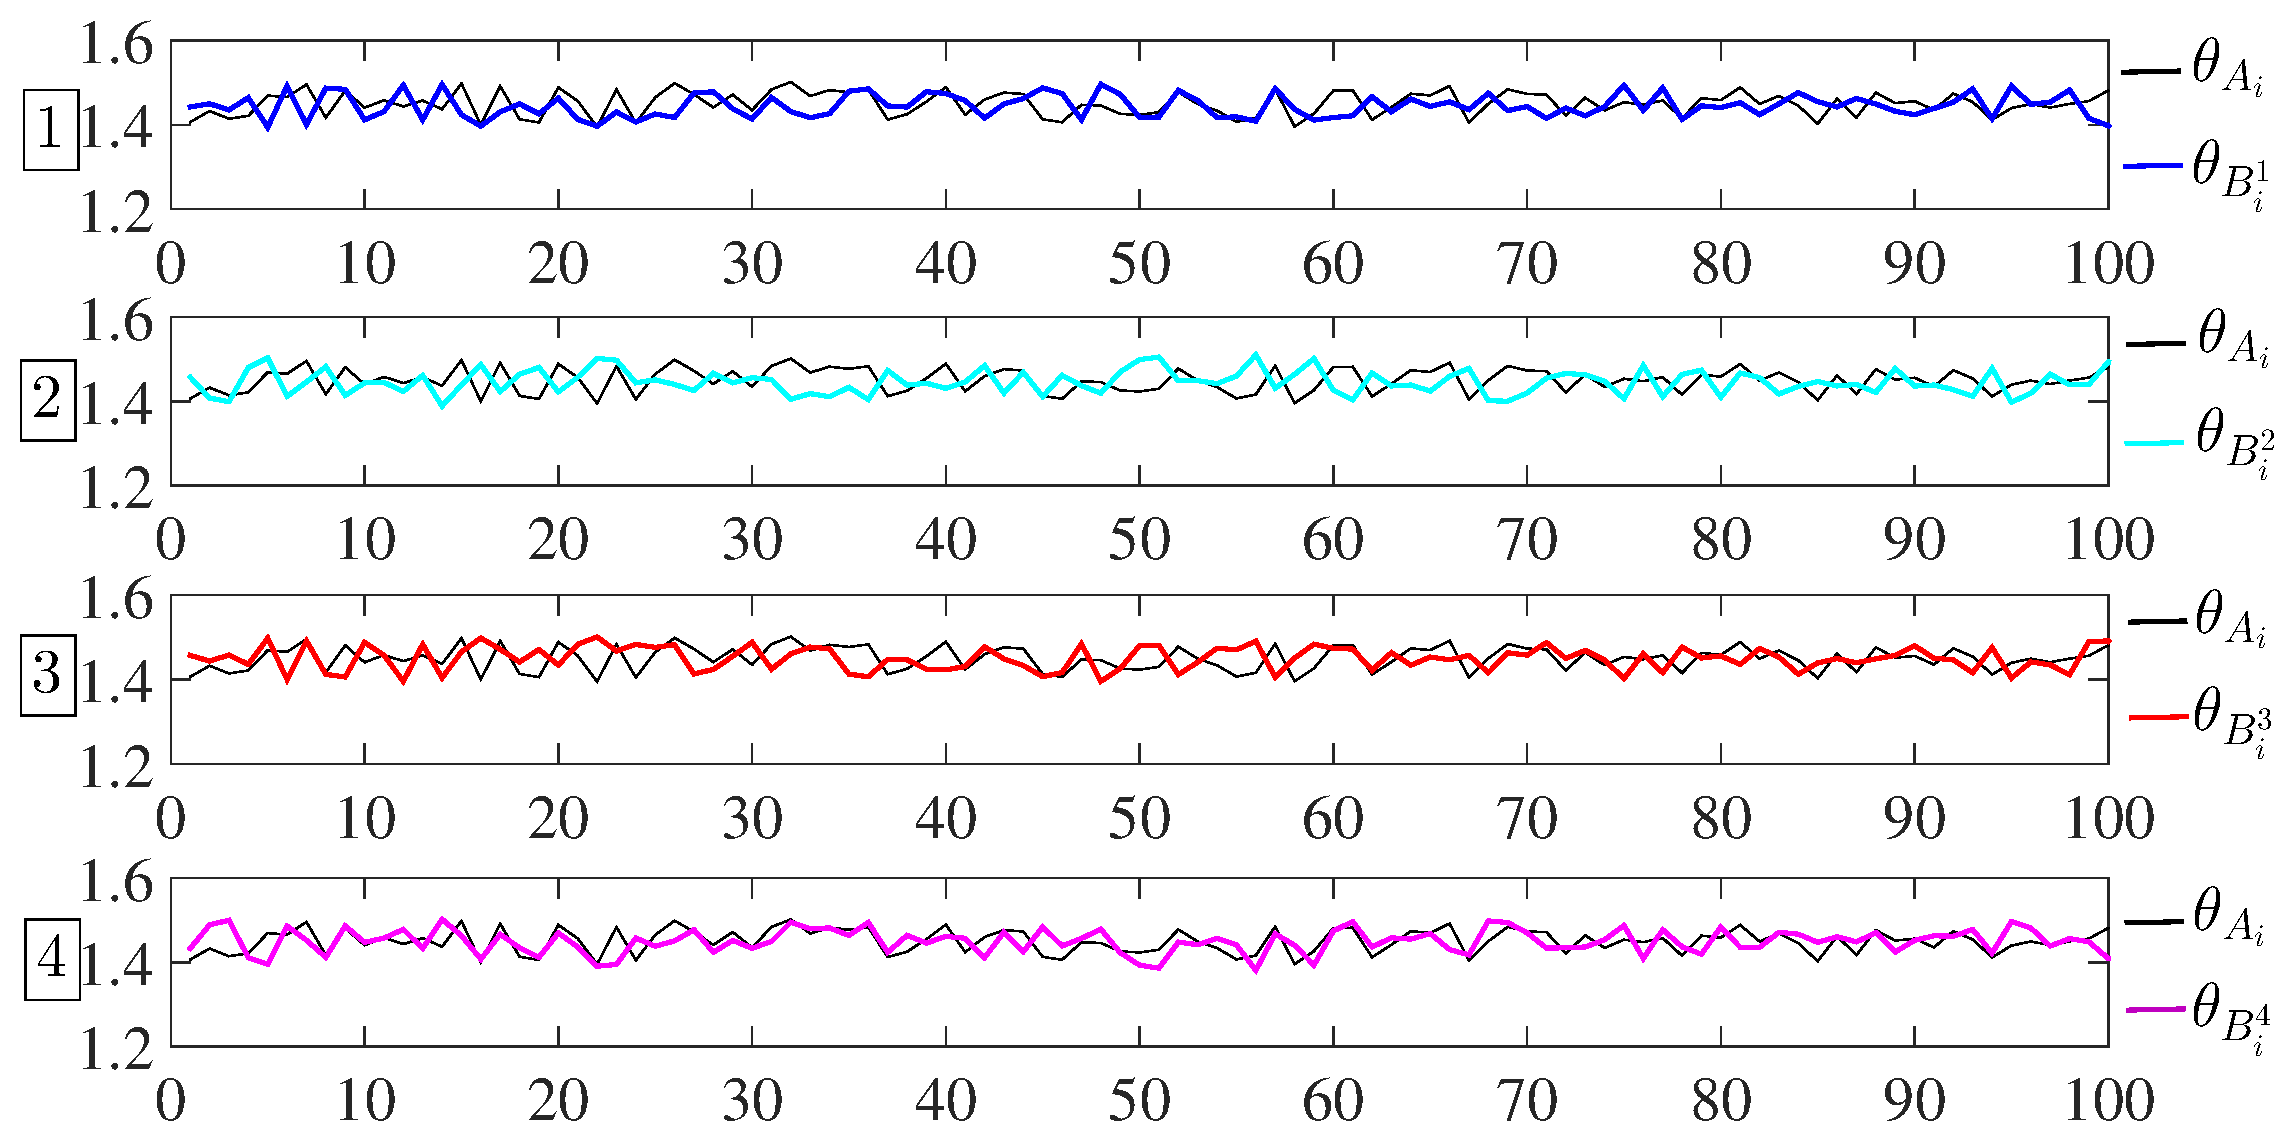
\includegraphics[width=3.2in]{fig7.eps}
\caption{
$Error(R_Y)$ distribution as the $As$ and $Bs$ spread ($\sigma(x_i) = 0.1, 0.2, 0.4, 0.6, 0.8, 1, 2$ as shown in Fig.~\ref{fig2})
}
\label{fig7}
\end{figure}
\end{center}

\begin{center}
\begin{figure}
\centering
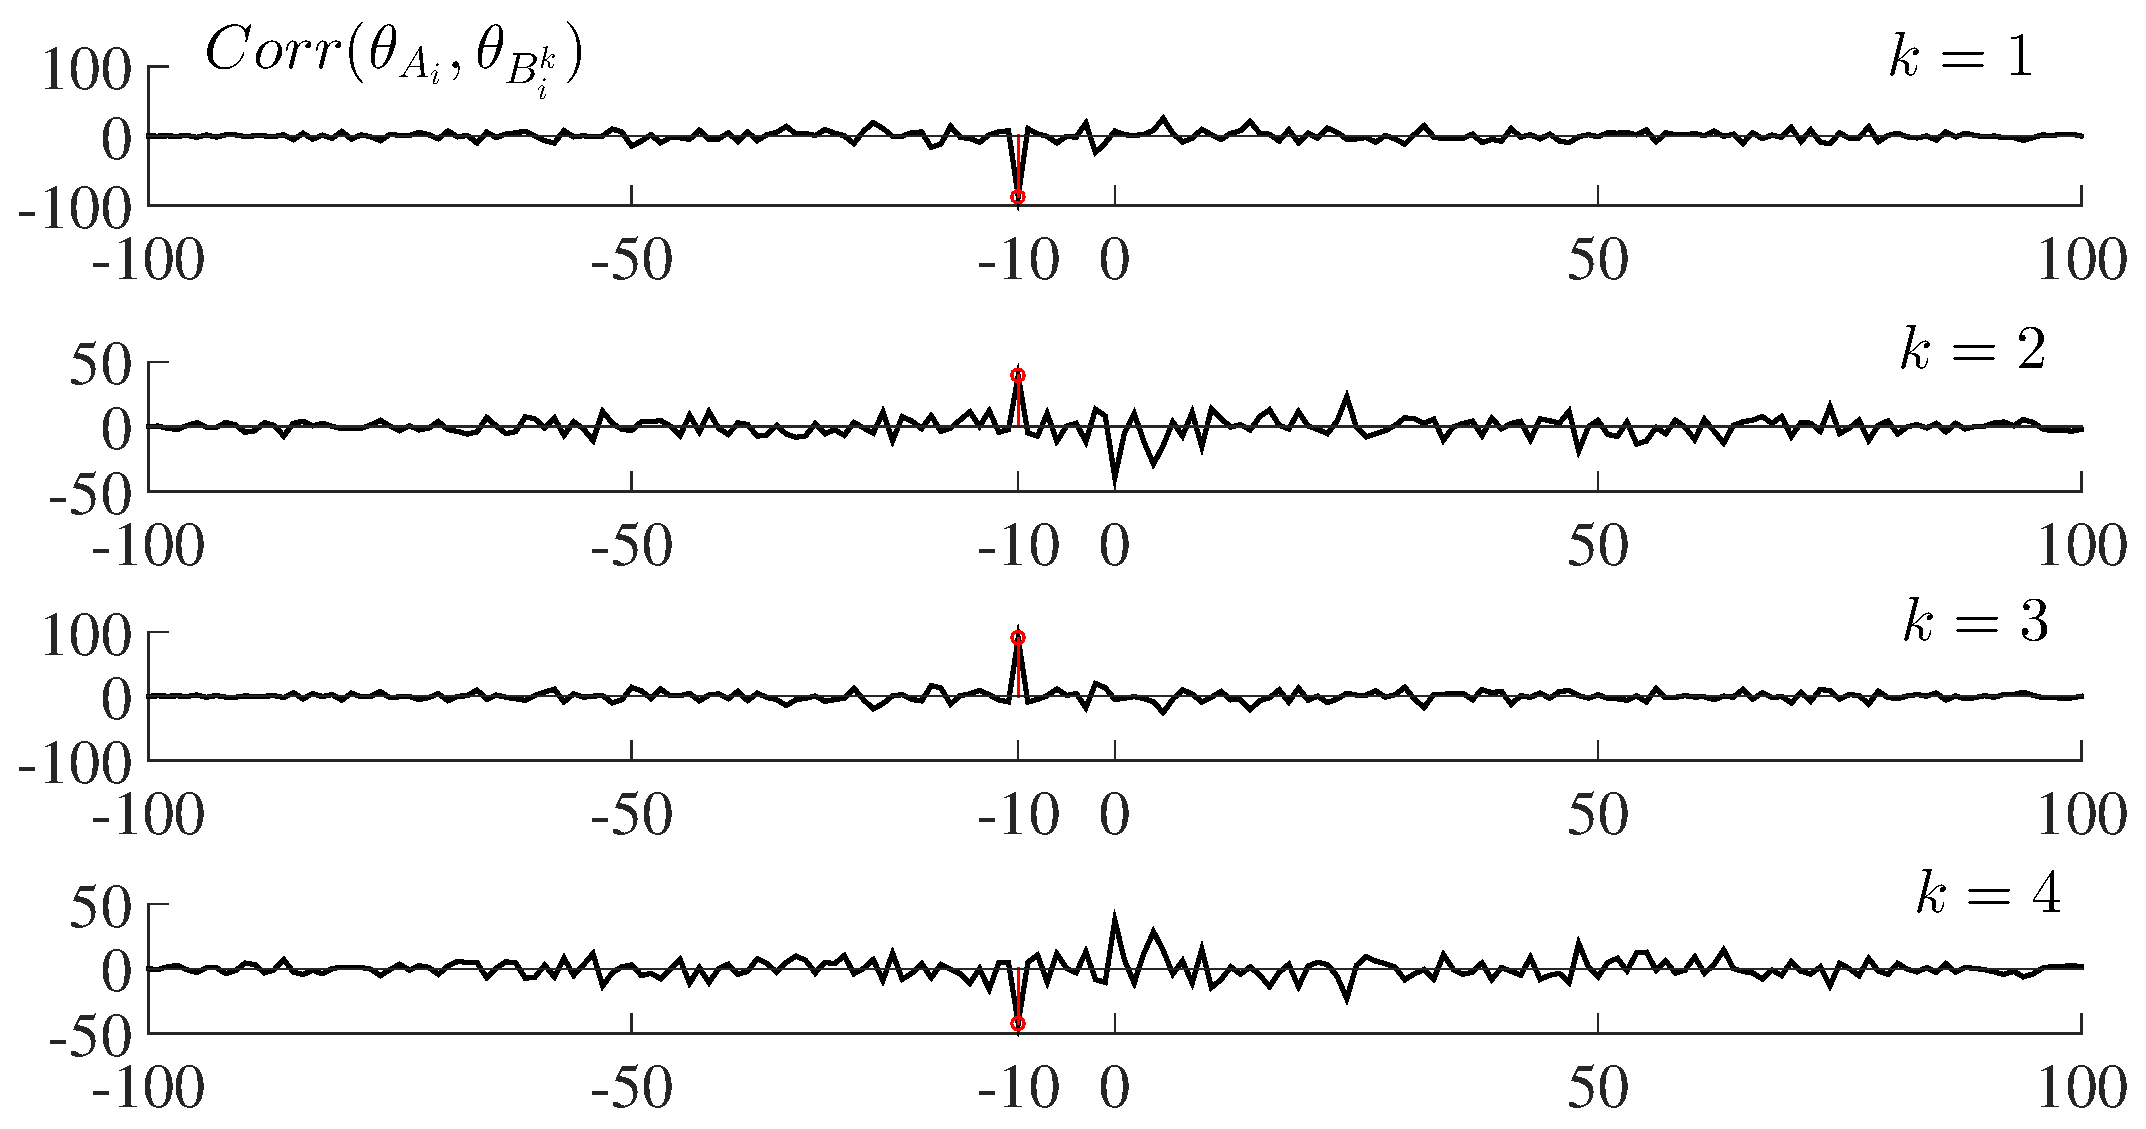
\includegraphics[width=3.2in]{fig8.eps}
\caption{
$Error(t_X)$ distribution as the $As$ and $Bs$ spread ($\sigma(x_i) = 0.1, 0.2, 0.4, 0.6, 0.8, 1, 2$ as shown in Fig.~\ref{fig2})
}
\label{fig8}
\end{figure}
\end{center}

\begin{center}
\begin{figure}
\centering
\includegraphics[width=3.2in]{fig9.eps}
\caption{
$Error(t_Y)$ distribution as the $As$ and $Bs$ spread ($\sigma(x_i) = 0.1, 0.2, 0.4, 0.6, 0.8, 1, 2$ as shown in Fig.~\ref{fig2})
}
\label{fig9}
\end{figure}
\end{center}


In the generation of $B_i = B_{init} exp(\mathbf{\widehat{x}})$, each element $x_j$ of $\mathbf{x} = (x_1,x_2,x_3,x_4,x_5,x_6)^T $ is Gaussian with $N \sim (\mu,\sigma)$. Small disturbances are exerted to the $B_i$ to make the noisy $B_i^{noise} = B_i exp(\mathbf{\widehat{x}}_{noise})$, where each of Lie Algebra element of $\mathbf{x}$ is Gaussian distribution $N \sim (\mu_{noise},\sigma_{noise})$. In Fig.~\ref{fig8},~\ref{fig9},~\ref{fig10} and~\ref{fig11}, $\sigma_{noise}$ is 0.005. As $\sigma$ varies from $0.1$ to $2$, the errors of $R_X$, $R_Y$, $t_X$, and $t_Y$ are reduced as shown in the box-and-whisker plot. There are several outliers not included between the whiskers. The median data can be used as the final solved $X$ and $Y$.



\begin{center}
\begin{figure}
\centering
\includegraphics[width=2.6in]{fig10.eps}
\caption{
The distribution of solved $X$.
}
\label{fig10}
\end{figure}
\end{center}

\begin{center}
\begin{figure}
\centering
\includegraphics[width=2.6in]{fig11.eps}
\caption{
The distribution of solved $Y$.
}
\label{fig11}
\end{figure}
\end{center}

\section{Conclusions}
\label{sect5}

In this paper, we developed a probabilistic approach to simultaneously obtain  $X$ and $Y$ in $AX=YB$ sensor calibration problem. Without a prior knowledge of the correspondence between $A$ and $B$, in the algorithm the probability theory in Lie group is used to constrain the solution of $X$ and $Y$ to eight candidates. As for the shifted data stream of $A$ and $B$, using the correlation theorem with Euclidean group invariants,the correspondence is recovered to determine the correct solution from eight candidates. In numeric simulation, the method perform well with different data samples.
%\section{Conclusion}
% conference papers do not normally have an appendix

\addtolength{\textheight}{-12cm}   % This command serves to balance the column lengths
                                  % on the last page of the document manually. It shortens
                                  % the textheight of the last page by a suitable amount.
                                  % This command does not take effect until the next page
                                  % so it should come on the page before the last. Make
                                  % sure that you do not shorten the textheight too much.

%%%%%%%%%%%%%%%%%%%%%%%%%%%%%%%%%%%%%%%%%%%%%%%%%%%%%%%%%%%%%%%%%%%%%%%%%%%%%%%%



%%%%%%%%%%%%%%%%%%%%%%%%%%%%%%%%%%%%%%%%%%%%%%%%%%%%%%%%%%%%%%%%%%%%%%%%%%%%%%%%



%%%%%%%%%%%%%%%%%%%%%%%%%%%%%%%%%%%%%%%%%%%%%%%%%%%%%%%%%%%%%%%%%%%%%%%%%%%%%%%%
\section*{APPENDIX}



\section*{ACKNOWLEDGMENT}



%%%%%%%%%%%%%%%%%%%%%%%%%%%%%%%%%%%%%%%%%%%%%%%%%%%%%%%%%%%%%%%%%%%%%%%%%%%%%%%%


\bibliographystyle{IEEEtran}
\bibliography{IEEEabrv,bibIEEEfull}
%\begin{thebibliography}{1}
%
%
%\end{thebibliography}

\end{document}
